\documentclass{article}
\usepackage{algpseudocode}
\usepackage{amsmath}
\usepackage{graphicx}
\usepackage{tabularx}
\usepackage{geometry}
\geometry{margin=1in}
\begin{document}
\title{Homework 2 Report}
\author{Yige Hu and Zhiting Zhu}
\date{}
\maketitle

% declaration of the new block
\algblock{ParFor}{EndParFor}
% customising the new block
\algnewcommand\algorithmicparfor{\textbf{parfor}}
\algnewcommand\algorithmicpardo{\textbf{do}}
\algnewcommand\algorithmicendparfor{\textbf{end\ parfor}}
\algrenewtext{ParFor}[1]{\algorithmicparfor\ #1\ \algorithmicpardo}
\algrenewtext{EndParFor}{\algorithmicendparfor}

\section{P1}
\begin{algorithmic}[1]
  \Function{rec\_psum}{$a, x_0, b, n$} \label{alg:a}
\item[]
  \If{(n == 1)}
  \State $s(0) = x_0; return; end;$
  \EndIf
\item[]
  \State $x = zeros(n/2, 1);$
  \State $a\_new = zeros(n/2 - 1, 1);$
  \State $x(0) = x_0;$
  \ParFor{$i = 1 : n$}
  \State $x(i) = b(i);$
  \EndParFor
\item[]
  \ParFor{$i = 0 : n/2 - 1$}
  \State $y(i) = x(2*i) * a(2*i+1) + x(2*i+1);$
  \If{(i != 0)}
  \State $a\_new(i) = a(2*i) * a(2*i+1);$
  \EndIf
  \EndParFor
\item[]
  \State $c = $ \Call{rec\_psum}{$a\_new, y(0), y[1 : n/2 - 1], n/2$} $;$
\item[]
  \State $s(0) = x_0;$
  \ParFor{$i = 1 : n - 1$}
  \If{isOdd(i)}
  \State $s(i) = c(i/2);$
  \Else
  \State $s(i) = c((i-1)/2) * a(i) + x(i);$
  \EndIf
  \EndParFor
\item[]
  \State \Return $s;$
  \EndFunction
\end{algorithmic}

\section{P2}
\subsection{Algorithm}
\begin{algorithmic}[1]
  \Function{scan}{$x, n, l$}\label{alg:p2}
\item[]
  \State $step = ceil(log_2(n))$
  \State $temp = n >> 1$
  \State $offset = 1$
\item[]
  \ParFor {$i=0:n/2-1$}
  \For {$j=i; j < temp; j += nthreads$}
  \State $indx2 = offset*(2*i+2)-1$
  \State $indx1 = offset*(2*i+1)-1$
  \State $x(indx2) = x(indx1)+x(indx2)$
  \EndFor
  \State $offset *= 2$
  \State $temp = temp >> 1$
  \EndParFor
\item[]
  \State $temp = 2$
  \State $offset >>= 1$
\item[]
  \ParFor {$i=1:n/2-1$}
  \State $offset >>= 1$
  \For {$j=i; j < temp; j += nthreads$}
  \State $indx2 = offset*(2*i+1)-1$
  \State $indx1 = offset*2*i-1$
  \State $x(indx2) = x(indx1)+x(indx2)$
  \EndFor
  \State $temp *= 2$
  \EndParFor 
  \EndFunction
\end{algorithmic}

\subsection{Result}
\begin{table}[h]
  \centering
  \begin{tabular}{|c|c|c|c|}
    \hline
    Wall Clock Time(us) & \multicolumn{3}{|c|}{Number of threads} \\
    \hline
    Length of Arrary & sequential & 6 threads & 12 threads \\
    \hline
    1M	& 15679	& 15500	& 38192 \\
    \hline
    10M	& 156797.9 & 212012.5 &	160871 \\
    \hline
    100M & 730794.8 & 1513714 &	1262623.5 \\
    \hline
    1B & 7305516.5 & 14843186 &	12431315.5 \\
    \hline
  \end{tabular}
  \caption{Wall clock execution time for different array size with different
    number of threads for 1D vectors}
  \label{table:1D_p2}
\end{table}

\begin{figure}[h]
  \centering
  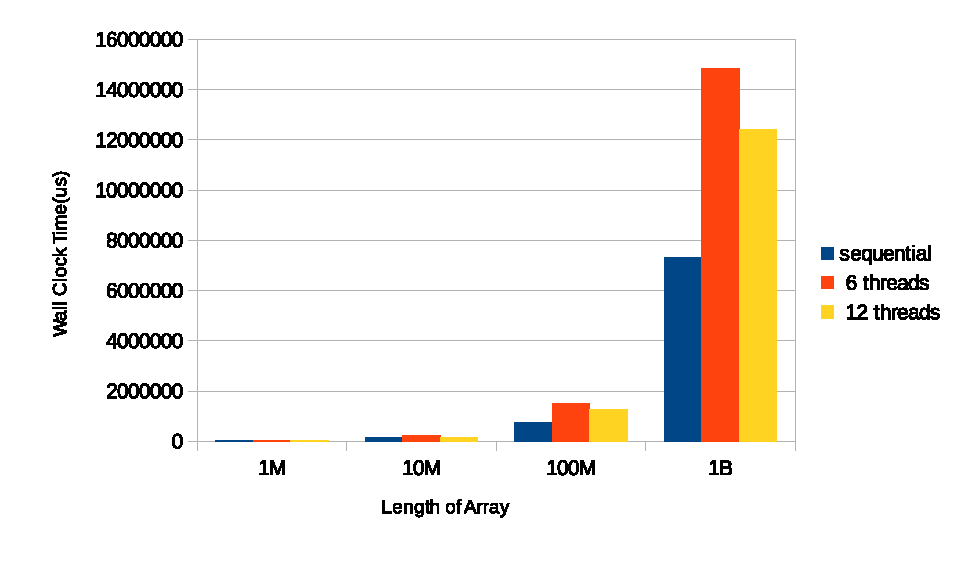
\includegraphics[width=\textwidth]{fig/1D_p2}
  \caption{Wall clock execution time for different array size with
    different number of threads for 1D
    vectors}
  \label{fig:1D_p2}
\end{figure}

\begin{table}[h]
  \centering
  \begin{tabular}{|c|c|c|c|}
    \hline
    Wall Clock Time(us) & \multicolumn{3}{|c|}{Number of threads} \\
    \hline
    Length of Arrary & sequential & 6 threads & 12 threads \\
    \hline
    1M & 20525.5 & 79923.5 & 146187 \\
    \hline
    10M	& 247284.5 & 539063 & 375131.5 \\
    \hline
    100M & 2046770 & 4615023.5 & 3381959 \\
    \hline
  \end{tabular}
  \caption{Wall clock execution time for different array size with different
    number of threads for 4D vectors}
  \label{table:4D_p2}
\end{table}

\begin{figure}[h]
  \centering
  \includegraphics[width=\textwidth]{fig/4D_p2}
  \caption{Timing measurements for different array size with different
    number of threads for 4D vectors}
  \label{fig:4D_p2}
\end{figure}


\section{P3}

\end{document}
